% ============================================================
%  formulario_electromagnetismo.tex
%  Formulario de Electromagnetismo — Un tema por página
%  Mathwizards Consultoría Educativa STEM
%
%  Compilar:  latexmk -xelatex formulario_electromagnetismo.tex
% ============================================================
\documentclass[9pt, landscape, letterpaper]{extarticle}
\usepackage{mathwizards-formulario}

\mwformulario{Formulario de Electromagnetismo}{Mathwizards $\cdot$ Física}

\begin{document}

% ════════════════════════════════════════════════════════════
%  PÁGINA 1 — Fundamentos y Herramientas Matemáticas / Fuerzas fundamentales
% ════════════════════════════════════════════════════════════
\nuevotema{Fundamentos y Herramientas Matemáticas / Fuerzas Fundamentales, Trabajo y Cinemática}

\begin{multicols}{4}

  % --- Prefijos de Ingeniería ---
  \subsection{Prefijos de Ingeniería}

  \begin{tablabox}[Submúltiplos]
    \tablacompacta
    \begin{tabular}{@{}lcc@{}}
      \toprule
      Prefijo & Símb. & Factor            \\
      \midrule
      deci    & d     & $\times 10^{-1}$  \\
      centi   & c     & $\times 10^{-2}$  \\
      mili    & m     & $\times 10^{-3}$  \\
      micro   & $\mu$ & $\times 10^{-6}$  \\
      nano    & n     & $\times 10^{-9}$  \\
      pico    & p     & $\times 10^{-12}$ \\
      femto   & f     & $\times 10^{-15}$ \\
      \bottomrule
    \end{tabular}
  \end{tablabox}

  \begin{tablabox}[Múltiplos]
    \tablacompacta
    \begin{tabular}{@{}lcc@{}}
      \toprule
      Prefijo & Símb. & Factor          \\
      \midrule
      kilo    & k     & $\times 10^{3}$ \\
      mega    & M     & $\times 10^{6}$ \\
      giga    & G     & $\times 10^{9}$ \\
      \bottomrule
    \end{tabular}
  \end{tablabox}

  % --- Coordenadas y Distancia ---
  \subsection{Coordenadas y Distancia}

  \begin{formulabox}
    $$\alpha = \tan^{-1}\!\left(\frac{y}{x}\right)$$
    $$d = \sqrt{(y_2 - y_1)^2 + (x_2 - x_1)^2}$$
  \end{formulabox}

  % --- Pitágoras ---
  \subsection{Teorema de Pitágoras}

  \begin{formulabox}
    $$c = \sqrt{a^2 + b^2}$$
    $$a = \sqrt{c^2 - b^2} \quad b = \sqrt{c^2 - a^2}$$
  \end{formulabox}

  \begin{despejesbox}[Isósceles rectángulo]
    $$x = \sqrt{\frac{c^2}{2}} \quad c = \sqrt{2x^2}$$
  \end{despejesbox}

  % --- Seno y Coseno ---
  \subsection{Teoremas del Seno y Coseno}

  \begin{formulabox}[Ley de Cosenos]
    \begin{align*}
      a & = \sqrt{b^2 + c^2 - 2bc\cos\alpha} \\
      b & = \sqrt{a^2 + c^2 - 2ac\cos\beta}  \\
      c & = \sqrt{a^2 + b^2 - 2ab\cos\gamma}
    \end{align*}
    \vspace{-8pt}
  \end{formulabox}

  \begin{formulabox}[Ley de Senos]
    $$\frac{\sen\alpha}{a} = \frac{\sen\beta}{b} = \frac{\sen\gamma}{c}$$
  \end{formulabox}

  \begin{despejesbox}[Ángulos]
    \begin{align*}
      \alpha & = \cos^{-1}\!\left(\frac{-a^2 + b^2 + c^2}{2bc}\right) \\
      \beta  & = \cos^{-1}\!\left(\frac{-b^2 + a^2 + c^2}{2ac}\right) \\
      \gamma & = \cos^{-1}\!\left(\frac{-c^2 + a^2 + b^2}{2ab}\right)
    \end{align*}
    \vspace{-8pt}
  \end{despejesbox}

  % --- Descomposición Vectorial ---
  \subsection{Descomposición Vectorial}

  \begin{formulabox}[Componentes Rectangulares]
    \vspace{-4pt}
    $$\vec{A} = A_x\,\hat{\imath} + A_y\,\hat{\jmath} \qquad |\vec{A}| = \sqrt{A_x^2 + A_y^2}$$
    $$A_x = |\vec{A}|\cos\theta \qquad A_y = |\vec{A}|\sen\theta$$
    \vspace{-6pt}
  \end{formulabox}

  \begin{tablabox}[Corrección de Cuadrante ($\theta_0 = \tan^{-1}\!\left|\frac{A_y}{A_x}\right|$)]
    \tablacompacta
    \begin{tabular}{@{}ccc@{}}
      \toprule
      Cuad. & Signos $(A_x, A_y)$ & Dirección Real $\theta$         \\
      \midrule
      I     & $(+, +)$            & $\theta = \theta_0$             \\
      II    & $(-, +)$            & $\theta = 180^\circ - \theta_0$ \\
      III   & $(-, -)$            & $\theta = 180^\circ + \theta_0$ \\
      IV    & $(+, -)$            & $\theta = 360^\circ - \theta_0$ \\
      \bottomrule
    \end{tabular}
  \end{tablabox}

  \begin{notabox}[Calculadora: $\mathrm{Rec}$ y $\mathrm{Pol}$]
    \centering\footnotesize
    \textbf{Rec}$(|\vec{A}|,\, \theta) \;\to\; X = A_x,\; Y = A_y$ \quad {\scriptsize(\texttt{SHIFT} \texttt{[-]})} \\[2pt]
    \textbf{Pol}$(A_x,\, A_y) \;\to\; r = |\vec{A}|,\; \theta$ \quad {\scriptsize(\texttt{SHIFT} \texttt{[+]})} \\[1pt]
    {\scriptsize\textit{($\mathrm{Pol}$ entrega el ángulo con signo y cuadrante correcto)}}
  \end{notabox}

  % --- Áreas ---
  \subsection{Áreas de Figuras Comunes}

  \begin{formulabox}
    $$A = \pi r^2 \quad A = b \cdot h \quad A = l^2$$
  \end{formulabox}

  % --- Partículas Subatómicas ---
  \subsection{Partículas Subatómicas}

  \begin{tablabox}
    \tablacompacta
    \begin{tabular}{@{}lll@{}}
      \toprule
      Part. & Masa                         & Carga                        \\
      \midrule
      $e^-$ & $9{,}11 \times 10^{-31}$ kg  & $-1{,}602 \times 10^{-19}$ C \\
      $p^+$ & $1{,}673 \times 10^{-27}$ kg & $+1{,}602 \times 10^{-19}$ C \\
      $n^0$ & $1{,}675 \times 10^{-27}$ kg & $0$                          \\
      \bottomrule
    \end{tabular}
  \end{tablabox}

  % --- Ley de Coulomb ---
  \subsection{Ley de Coulomb}

  \begin{formulabox}[Fuerza Eléctrica]
    $$\vec{F} = K \frac{q_1 \cdot q_2}{r^2}$$
  \end{formulabox}

  \begin{despejesbox}[Despejes]
    $$r = \sqrt{K \frac{q_1 \cdot q_2}{F}}$$
    $$q_1 = \frac{F\, r^2}{K\, q_2} \quad q_2 = \frac{F\, r^2}{K\, q_1}$$

    \textbf{Cargas iguales:}
    $$q = \sqrt{\frac{F \cdot r^2}{K}}$$
  \end{despejesbox}

  \begin{tablabox}[Variables]
    \tablacompacta
    \begin{tabular}{@{}lcl@{}}
      \toprule
      Símb.      & Descripción      & Unidad                                         \\
      \midrule
      $F$        & Fuerza Eléctrica & N                                              \\
      $K$        & Cte.\ de Coulomb & $9 \times 10^9 \frac{\text{Nm}^2}{\text{C}^2}$ \\
      $q_1, q_2$ & Cargas puntuales & C                                              \\
      $r$        & Distancia        & m                                              \\
      \bottomrule
    \end{tabular}
  \end{tablabox}

  \begin{notabox}[Principio de Cargas]
    \begin{itemize}
      \item Cargas iguales se \textbf{repelen}
      \item Cargas diferentes se \textbf{atraen}
    \end{itemize}
  \end{notabox}

  % --- Ley de Gravitación Universal ---
  \subsection{Gravitación Universal}

  \begin{formulabox}[Fuerza Gravitatoria]
    $$F = G \frac{m_1\, m_2}{r^2}$$
  \end{formulabox}

  \begin{despejesbox}[Despejes]
    $$r = \sqrt{G \frac{m_1\, m_2}{F}}$$
    $$m_1 = \frac{F\, r^2}{G\, m_2} \quad m_2 = \frac{F\, r^2}{G\, m_1}$$
  \end{despejesbox}

  \begin{tablabox}[Variables]
    \tablacompacta
    \begin{tabular}{@{}lcl@{}}
      \toprule
      Símb.      & Descripción         & Unidad                                                    \\
      \midrule
      $F$        & Fuerza Gravitatoria & N                                                         \\
      $G$        & Cte.\ gravitacional & $6{,}673 \times 10^{-11} \frac{\text{Nm}^2}{\text{kg}^2}$ \\
      $m_1, m_2$ & Masas               & kg                                                        \\
      $r$        & Distancia           & m                                                         \\
      \bottomrule
    \end{tabular}
  \end{tablabox}

  % --- Fuerza y Peso ---
  \subsection{Segunda Ley de Newton}

  \begin{formulabox}
    $$\vec{F} = m \cdot \vec{a}$$
    $$m = \frac{F}{a} \quad a = \frac{F}{m}$$
  \end{formulabox}

  \subsection{Peso}

  \begin{formulabox}[Fuerza gravitatoria en la Tierra]
    $$P = m \cdot g$$
    $$m = \frac{P}{g} \qquad g = 9{,}81\ \text{m/s}^2$$
  \end{formulabox}

  % --- Trabajo ---
  % \subsection{Trabajo y Energía Interna}

  % \begin{formulabox
  % $$W = E_p - U$
  % \end{formulabox}

  % \begin{tablabox}[Variables]
  % \tablacompacta
  % \begin{tabular}{@{}lcl@{}}
  % \toprule
  % Símb. & Descripción       & Unidad \\
  % \midrule
  %      $W$   & Trabajo           & J      \\
  %     $E_p$ & Energía Potencial & J      \\
  %    $U$   & Energía Interna   & J      \\
  %   \bottomrule
  %\end{tabular}
  % \end{tablabox}

  % --- Cinemática ---
  \subsection{MRU}

  \begin{formulabox}
    $$x = V \cdot t$$
  \end{formulabox}

  \subsection{MRUV}

  \begin{formulabox}
    \begin{align*}
      V_f   & = V_0 + a \cdot t            \\
      d     & = V_0 t + \tfrac{1}{2} a t^2 \\
      V_f^2 & = V_0^2 + 2 a d
    \end{align*}
    \vspace{-8pt}
  \end{formulabox}

\end{multicols}



% ════════════════════════════════════════════════════════════
%  PÁGINA 2 — Campos Eléctricos y Potencial Eléctrico / Capacitancia Eléctrica
% ════════════════════════════════════════════════════════════
\nuevotema{Campos Eléctricos y Potencial Eléctrico / Capacitancia Eléctrica / Asociación de Capacitores}

\begin{multicols}{4}

  % --- Campos Eléctricos ---
  \subsection{Definición por Fuerza}

  \begin{formulabox}
    $$\vec{E} = \frac{\vec{F}}{q} \qquad q = \frac{F}{E} \qquad \vec{F} = \vec{E} \cdot q$$
  \end{formulabox}

  \subsection{Campo de Carga Puntual}

  \begin{formulabox}
    $$E = \frac{K \cdot q}{r^2}$$
  \end{formulabox}

  \begin{despejesbox}[Despejes]
    $$r = \sqrt{\frac{K \cdot q}{E}} \quad q = \frac{E \cdot r^2}{K}$$
  \end{despejesbox}

  \subsection{Campo con Dieléctrico}

  \begin{formulabox}
    $$E = \frac{K \cdot q}{\varepsilon \cdot r^2}$$
  \end{formulabox}

  \subsection{Relación Campo--Potencial}

  \begin{formulabox}
    $$E = \frac{V}{r} \qquad V = E \cdot r$$
  \end{formulabox}

  \subsection{Valores Característicos de $E$}

  \begin{tablabox}
    \tablacompacta
    \begin{tabular}{@{}p{3.2cm}r@{}}
      \toprule
      Situación           & $E$ (N/C)          \\
      \midrule
      Tubo fluorescente   & $10^1$             \\
      Atmósfera           & $10^2$             \\
      Regla/globo cargado & $10^3$             \\
      Fotocopiadora       & $10^5$             \\
      Descarga en aire    & $> 3 \times 10^6$  \\
      Electrón en H       & $5 \times 10^{11}$ \\
      Núcleo de U         & $3 \times 10^{21}$ \\
      \bottomrule
    \end{tabular}
  \end{tablabox}

  % --- Potencial Eléctrico ---
  \subsection{Potencial de carga generadora}

  \begin{formulabox}
    $$V = \frac{K \cdot q}{r}$$
  \end{formulabox}

  \begin{despejesbox}[Despejes]
    $$r = \frac{K \cdot q}{V} \qquad q = \frac{V \cdot r}{K}$$
  \end{despejesbox}

  \subsection{Energía Potencial Eléctrica}

  \begin{formulabox}
    $$E_p = V \cdot q \quad V = \frac{E_p}{q} \quad q = \frac{E_p}{V}$$
  \end{formulabox}

  \subsection{Fórmulas Derivadas}

  \begin{despejesbox}[Cadena de igualdades]
    $$E = \frac{F}{q} = \frac{m \cdot a}{q} = \frac{V}{r}$$
  \end{despejesbox}

  \begin{despejesbox}[Despejes cruzados]
    $$q = \frac{F \cdot r}{V} \quad V = \frac{F \cdot r}{q} \quad r = \frac{q \cdot V}{F}$$
    $$a = \frac{V \cdot q}{r \cdot m} \quad m = \frac{E \cdot q}{a} \quad a = \frac{E \cdot q}{m}$$
  \end{despejesbox}

  \begin{formulabox}[Velocidad final]
    $$V_f = \sqrt{\frac{2 \cdot V \cdot q}{m} + V_0^2}$$
  \end{formulabox}

  \subsection{Variables}

  \begin{tablabox}
    \tablacompacta
    \begin{tabular}{@{}lcl@{}}
      \toprule
      Símb. & Descripción         & Unidad                                         \\
      \midrule
      $K$   & Cte.\ de Coulomb    & $9 \times 10^9 \frac{\text{Nm}^2}{\text{C}^2}$ \\
      $q$   & Carga               & C                                              \\
      $r$   & Distancia           & m                                              \\
      $E$   & Campo Eléctrico     & N/C                                            \\
      $E_p$ & Energía Potencial   & J                                              \\
      $V$   & Potencial Eléctrico & V                                              \\
      $a$   & Aceleración         & m/s$^2$                                        \\
      $m$   & Masa                & kg                                             \\
      \bottomrule
    \end{tabular}
  \end{tablabox}

  \subsection{Definición de Capacitancia}

  \begin{formulabox}
    $$C = \frac{q}{\Delta V}$$
    $$q = C \cdot \Delta V \qquad \Delta V = \frac{q}{C}$$
  \end{formulabox}

  \subsection{Capacitor de Placas Paralelas}

  \begin{formulabox}
    $$C = \frac{\varepsilon \cdot A}{4\pi \cdot k \cdot d}$$
  \end{formulabox}

  \begin{despejesbox}[Despeje]
    $$A = \frac{4\pi \cdot k \cdot C \cdot d}{\varepsilon}$$
  \end{despejesbox}

  \subsection{Fuerza con Dieléctrico}

  \begin{formulabox}
    $$F = \frac{K \cdot q_1 \cdot q_2}{\varepsilon \cdot r^2}$$
  \end{formulabox}

  \begin{despejesbox}[Despejes]
    $$q_1 = \frac{F \varepsilon\, r^2}{K\, q_2} \quad r = \sqrt{\frac{K q_1 q_2}{F \varepsilon}}$$
    $$q_2 = \frac{F \varepsilon\, r^2}{K\, q_1}$$
  \end{despejesbox}

  \subsection{Rigidez Eléctrica}

  \begin{formulabox}
    $$V_{\text{máx}} = RE \cdot d$$
    $$d = \frac{V_{\text{máx}}}{RE} \qquad RE = \frac{V_{\text{máx}}}{d}$$
  \end{formulabox}

  \begin{tablabox}[Variables]
    \tablacompacta
    \begin{tabular}{@{}lcl@{}}
      \toprule
      Símb.            & Descripción         & Unidad \\
      \midrule
      $d$              & Dist.\ entre placas & m      \\
      $V_{\text{máx}}$ & Voltaje máximo      & V      \\
      $RE$             & Rigidez Eléctrica   & V/m    \\
      \bottomrule
    \end{tabular}
  \end{tablabox}

  \subsection{Energía en Capacitor}

  \begin{formulabox}
    $$E_p = \frac{C \cdot (\Delta V)^2}{2}$$
  \end{formulabox}

  \begin{despejesbox}[Despejes]
    $$C = \frac{2 E_p}{(\Delta V)^2} \quad \Delta V = \sqrt{\frac{2 E_p}{C}}$$
  \end{despejesbox}

  \subsection{Potencia}

  \begin{formulabox}
    $$P = \frac{E_p}{t} \quad E_p = P \cdot t \quad t = \frac{E_p}{P}$$
  \end{formulabox}

  \begin{tablabox}[Variables]
    \tablacompacta
    \begin{tabular}{@{}lcl@{}}
      \toprule
      Símb. & Descripción       & Unidad \\
      \midrule
      $E_p$ & Energía Acumulada & J      \\
      $P$   & Potencia          & W      \\
      $t$   & Tiempo            & s      \\
      \bottomrule
    \end{tabular}
  \end{tablabox}
  \subsection{Constantes Dieléctricas y Rigidez}

  \begin{tablabox}
    \tablacompacta
    \begin{tabular}{@{}lcc@{}}
      \toprule
      Material      & $\varepsilon$ & $RE$ (V/m)                \\
      \midrule
      Aire seco     & 1,00054       & $3 \times 10^6$           \\
      Madera seca   & 1,5 -- 4      & ---                       \\
      Teflón        & 2,1           & $60 \times 10^6$          \\
      Caucho        & 2,1 -- 2,9    & $(16$--$28) \times 10^6$  \\
      Aceite        & 2,24          & $12 \times 10^6$          \\
      Parafina      & 2,1 -- 2,5    & $10 \times 10^6$          \\
      Polietileno   & 2,26          & $(19$--$22) \times 10^6$  \\
      Poliestireno  & 2,6           & $24 \times 10^6$          \\
      Ebonita       & 2,8           & $28 \times 10^6$          \\
      Nieve         & 3,3           & ---                       \\
      Plexiglas     & 3,4           & $40 \times 10^6$          \\
      Papel         & 3,5 -- 3,7    & $16 \times 10^6$          \\
      Cuarzo        & 3,8           & $(25$--$40) \times 10^6$  \\
      Hielo         & 4,2           & $0{,}15 \times 10^6$      \\
      Pyrex         & 4,7 -- 5,6    & $14 \times 10^6$          \\
      Baquelita     & 4,9           & $24 \times 10^6$          \\
      Mica          & 5,4           & $(10$--$100) \times 10^6$ \\
      Vidrio        & 5,4 -- 10     & $118 \times 10^6$         \\
      Porcelana     & 5,7 -- 6,8    & $10 \times 10^6$          \\
      Neopreno      & 6,9           & $12 \times 10^6$          \\
      Etanol        & 25            & ---                       \\
      Agua (20\,°C) & 80,4          & ---                       \\
      \bottomrule
    \end{tabular}
  \end{tablabox}

  \subsection{Capacitores en Paralelo}

  \begin{formulabox}
    $$C_{\text{total}} = C_1 + C_2 + \cdots + C_n$$
    $$Q = q_1 + q_2 + \cdots + q_n$$
    $$\Delta V = \Delta V_1 = \Delta V_2 = \cdots = \Delta V_n$$
  \end{formulabox}

  \begin{despejesbox}[Carga individual]
    $$q_i = C_i \cdot \Delta V$$
  \end{despejesbox}

  \subsection{Capacitores en Serie}

  \begin{formulabox}
    $$\frac{1}{C_{\text{total}}} = \frac{1}{C_1} + \frac{1}{C_2} + \cdots + \frac{1}{C_n}$$
    $$Q = q_1 = q_2 = \cdots = q_n$$
    $$\Delta V = \Delta V_1 + \Delta V_2 + \cdots + \Delta V_n$$
  \end{formulabox}

\end{multicols}

% ════════════════════════════════════════════════════════════
%  PÁGINA 3 — Corriente Eléctrica y Resistividad / Ley de Ohm, Conexión de Resistencias y Leyes de Kirchhoff
% ════════════════════════════════════════════════════════════
\nuevotema{Corriente Eléctrica y Resistividad / Ley de Ohm, Conexión de Resistencias y Leyes de Kirchhoff}

\begin{multicols}{4}

  \subsection{Intensidad de Corriente}

  \begin{formulabox}
    $$I = \frac{\Delta Q}{\Delta t} \quad \Delta t = \frac{\Delta Q}{I} \quad \Delta Q = I \cdot \Delta t$$
  \end{formulabox}

  \subsection{Cargas y Electrones}

  \begin{formulabox}
    $$N_e = \frac{\Delta Q}{e} \qquad e = 1{,}602 \times 10^{-19}\ \text{C}$$
  \end{formulabox}

  \subsection{Energía Eléctrica}

  \begin{formulabox}
    $$E = P \cdot t \quad P = \frac{E}{t} \quad t = \frac{E}{P}$$
  \end{formulabox}


  \subsection{Resistividad}

  \begin{formulabox}
    $$R = \rho \frac{L}{S} \quad \rho = \frac{R \cdot S}{L}$$
    $$L = \frac{R \cdot S}{\rho} \quad S = \rho \frac{L}{R}$$
  \end{formulabox}

  \begin{despejesbox}[Área transversal circular]
    $$S = \frac{\pi d^2}{4} = \pi r^2$$
    $$r = \sqrt{\frac{S}{\pi}} \quad d = 2\sqrt{\frac{S}{\pi}}$$
  \end{despejesbox}

  \begin{tablabox}[Variables]
    \tablacompacta
    \begin{tabular}{@{}lcl@{}}
      \toprule
      Símb.   & Descripción          & Unidad          \\
      \midrule
      $R$     & Resistencia          & $\Omega$        \\
      $\rho$  & Resistividad         & $\Omega \cdot$m \\
      $L$     & Longitud             & m               \\
      $S$     & Área transversal     & m$^2$           \\
      $e$     & Carga electrón       & C               \\
      $N_{e}$ & Número de electrones & adim.           \\
      \bottomrule
    \end{tabular}
  \end{tablabox}

  \subsection{Tabla de Resistividad (23\,°C)}

  \begin{tablabox}
    \tablacompacta
    \begin{tabular}{@{}lr@{}}
      \toprule
      Material       & $\rho$ ($\Omega \cdot$m)   \\
      \midrule
      Plata          & $1{,}59 \times 10^{-8}$    \\
      Cobre          & $1{,}68 \times 10^{-8}$    \\
      Oro            & $2{,}20 \times 10^{-8}$    \\
      Aluminio       & $2{,}65 \times 10^{-8}$    \\
      Tungsteno      & $5{,}6 \times 10^{-8}$     \\
      Hierro         & $9{,}71 \times 10^{-8}$    \\
      Platino        & $1{,}1 \times 10^{-7}$     \\
      Plomo          & $2{,}2 \times 10^{-7}$     \\
      Acero          & $7{,}2 \times 10^{-7}$     \\
      Nicromio       & $1{,}50 \times 10^{-6}$    \\
      Carbón         & $3{,}5 \times 10^{-5}$     \\
      Germanio       & $4{,}6 \times 10^{-1}$     \\
      Silicio        & $6{,}40 \times 10^{2}$     \\
      Piel humana    & $\sim 5{,}0 \times 10^{3}$ \\
      Vidrio         & $10^{10}$ -- $10^{14}$     \\
      Hule           & $\sim 10^{13}$             \\
      Sulfuro        & $10^{15}$                  \\
      Cuarzo (fund.) & $7{,}5 \times 10^{17}$     \\
      \bottomrule
    \end{tabular}
  \end{tablabox}

  % --- Rueda de Ohm ---
  \subsection{Rueda de la Ley de Ohm}

  \begin{tablabox}[Potencia $P$ (W)]
    \tablacompacta
    $$P = \frac{V^2}{R} = I^2 R = V \cdot I$$
  \end{tablabox}

  \begin{tablabox}[Intensidad $I$ (A)]
    \tablacompacta
    $$I = \frac{V}{R} = \sqrt{\frac{P}{R}} = \frac{P}{V}$$
  \end{tablabox}

  \begin{tablabox}[Voltaje $V$ (V)]
    \tablacompacta
    $$V = \sqrt{P \cdot R} = \frac{P}{I} = I \cdot R$$
  \end{tablabox}

  \begin{tablabox}[Resistencia $R$ ($\Omega$)]
    \tablacompacta
    $$R = \frac{P}{I^2} = \frac{V^2}{P} = \frac{V}{I}$$
  \end{tablabox}

  % --- Conexión de Resistencias ---
  \subsection{Resistencias en Serie}

  \begin{formulabox}
    $$V_{\text{total}} = V_1 + V_2 + \cdots + V_n$$
    $$R_{\text{total}} = R_1 + R_2 + \cdots + R_n$$
    $$I_{\text{total}} = I_1 = I_2 = \cdots = I_n$$
  \end{formulabox}

  \subsection{Resistencias en Paralelo}

  \begin{formulabox}
    $$V_{\text{total}} = V_1 = V_2 = \cdots = V_n$$
    $$\frac{1}{R_{\text{total}}} = \frac{1}{R_1} + \frac{1}{R_2} + \cdots + \frac{1}{R_n}$$
    $$I_{\text{total}} = I_1 + I_2 + \cdots + I_n$$
  \end{formulabox}

  % --- Kirchhoff ---
  % \subsection{Unidades y Equivalencias}
  %
  % \begin{tablabox}
  %  \tablacompacta
  % \begin{tabular}{@{}lp{4.5cm}@{}}
  %  \toprule
  % Magnitud & Equivalencias                                                                                                             \\
  %\midrule
  %$\Omega$ & $= \frac{V}{A} = \frac{W}{A^2} = \frac{V^2}{W} = \frac{\text{kg}\cdot\text{m}^2}{\text{s}^3 \cdot A^2}$                   \\[3pt]
  %V        & $= \frac{W}{A} = \frac{J}{C} = \frac{N\cdot\text{m}}{A\cdot\text{s}} = \frac{\text{kg}\cdot\text{m}^2}{A\cdot\text{s}^3}$ \\[3pt]
  %A        & $= \frac{C}{s}$                                                                                                           \\
  %\bottomrule
  %\end{tabular}
  %\end{tablabox}

  \subsection{1.ª Ley de Kirchhoff — Nodos}

  \begin{formulabox}
    $$\sum I_{\text{entrantes}} - \sum I_{\text{salientes}} = 0$$
  \end{formulabox}

  \begin{notabox}[Regla]
    \begin{itemize}
      \item Corrientes \textbf{entrantes}: $(+)$
      \item Corrientes \textbf{salientes}: $(-)$
    \end{itemize}
  \end{notabox}

  \subsection{2.ª Ley de Kirchhoff — Mallas}

  \begin{formulabox}
    $$\sum I \cdot R = \sum V$$
  \end{formulabox}

  \subsection{Criterio de Signos}

  \begin{center}
    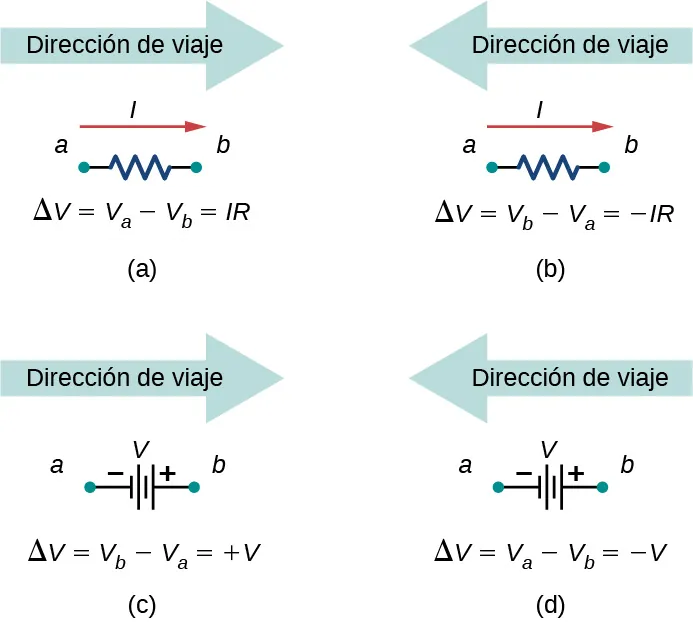
\includegraphics[width=0.95\linewidth]{kirchoff.png}
  \end{center}

  \begin{notabox}[Convenciones]
    \begin{itemize}
      \item Fuentes: $+V_{\text{em}}$ de $-$ a $+$;\; $-V_{\text{em}}$ de $+$ a $-$
      \item Resistencias: $IR$ si $I$ va en sentido de la malla
    \end{itemize}
  \end{notabox}

  %Tabla de Valores Caraterísticos

  \subsection{Valores Característicos (Voltaje)}

  \begin{tablabox}
    \tablacompacta
    \setlength{\tabcolsep}{-6pt}
    \begin{tabular}{@{}p{4.8cm}r@{}}
      \toprule
      Situación               & Voltaje        \\
      \midrule
      Electrocardiograma      & 5 mV           \\
      Pila de linterna        & 1,5 V          \\
      Batería de auto         & 12 V           \\
      Peligroso (piel húmeda) & 36 V           \\
      Peligroso (piel seca)   & 12 V           \\
      Red viviendas           & 110 / 220 V    \\
      Anguila eléctrica       & 600 V          \\
      Central eléctrica       & 26 kV          \\
      Descarga en aire        & 30 kV/cm       \\
      Tubo de pantalla        & 30 kV          \\
      Líneas transmisión      & 138--765 kV    \\
      Rayos atmosféricos      & $\leq 10^6$ kV \\
      \bottomrule
    \end{tabular}
  \end{tablabox}

  \subsection{Valores Característicos (Corriente)}

  \begin{tablabox}
    \tablacompacta
    \setlength{\tabcolsep}{-6pt}
    \begin{tabular}{@{}p{4.8cm}r@{}}
      \toprule
      Situación             & Intensidad        \\
      \midrule
      Mínimo detectable     & $\sim 10^{-17}$ A \\
      Impulso nervioso      & 10 $\mu$A         \\
      Base de transistor    & 10--100 $\mu$A    \\
      LED habitual          & 20--30 mA         \\
      Letal (cuerpo humano) & 0,1 A             \\
      Bombillo 60 W         & 0,5 A             \\
      Bombillo linterna 6 V & 0,8 A             \\
      Motor de agua         & 5 A               \\
      Hornilla eléctrica    & 5--9 A            \\
      Fusible vivienda      & 30 A              \\
      Rayo atmosférico      & 20 kA             \\
      \bottomrule
    \end{tabular}
  \end{tablabox}

  \subsection{Valores Característicos (Potencia)}

  \begin{tablabox}
    \tablacompacta
    \setlength{\tabcolsep}{-6pt}
    \begin{tabular}{@{}p{3.8cm}r@{}}
      \toprule
      Dispositivo        & Potencia    \\
      \midrule
      Auricular          & 5 mW        \\
      LED común          & 30 mW       \\
      Bombillo linterna  & 5 W         \\
      Lámpara ahorradora & 20 W        \\
      Fluorescentes      & 20--40 W    \\
      Filamento común    & 25--100 W   \\
      Abanico            & 60 W        \\
      Televisor          & 50--150 W   \\
      Refrigerador       & 180 W       \\
      Lavadora simple    & 360 W       \\
      Plancha eléctrica  & 300--1000 W \\
      Hornilla eléctrica & 600--1000 W \\
      Aire acondicionado & 1,5 kW      \\
      Centrales (1882)   & 12 kW       \\
      Termoeléctricas    & 1300 MW     \\
      \bottomrule
    \end{tabular}
  \end{tablabox}

\end{multicols}

% ════════════════════════════════════════════════════════════
%  PÁGINA 4 — Código de Colores y Constantes
% ════════════════════════════════════════════════════════════
\nuevotema{Código de Colores de Resistencias y Constantes Fundamentales / Introducción al Electromagnetismo}

\begin{multicols}{3}

  \subsection{Código de Colores}

  \begin{center}
    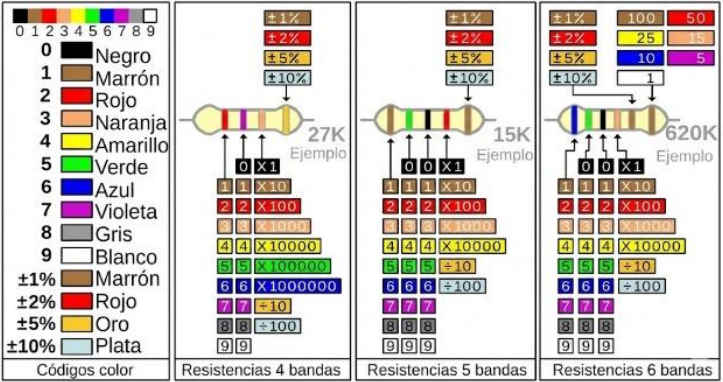
\includegraphics[width=0.9\linewidth]{colores_resistencias.png}
  \end{center}

  \begin{tablabox}[Tabla de Colores]
    \tablacompacta
    \begin{tabular}{@{}lccc@{}}
      \toprule
      Color    & Dígito & Multipl.        & Toler.         \\
      \midrule
      Negro    & 0      & $\times 1$      & ---            \\
      Marrón   & 1      & $\times 10$     & $\pm 1\%$      \\
      Rojo     & 2      & $\times 100$    & $\pm 2\%$      \\
      Naranja  & 3      & $\times 1$k     & ---            \\
      Amarillo & 4      & $\times 10$k    & ---            \\
      Verde    & 5      & $\times 100$k   & $\pm 0{,}5\%$  \\
      Azul     & 6      & $\times 1$M     & $\pm 0{,}25\%$ \\
      Violeta  & 7      & $\times 10$M    & $\pm 0{,}1\%$  \\
      Gris     & 8      & $\times 100$M   & $\pm 0{,}05\%$ \\
      Blanco   & 9      & $\times 1$G     & ---            \\
      Dorado   & ---    & $\times 0{,}1$  & $\pm 5\%$      \\
      Plateado & ---    & $\times 0{,}01$ & $\pm 10\%$     \\
      \bottomrule
    \end{tabular}
  \end{tablabox}

  \subsection{Constantes Fundamentales}

  \begin{tablabox}
    \tablacompacta
    \begin{tabular}{@{}lcl@{}}
      \toprule
      Cte.  & Valor                     & Unidad                            \\
      \midrule
      $K$   & $9 \times 10^9$           & $\frac{\text{Nm}^2}{\text{C}^2}$  \\[3pt]
      $G$   & $6{,}673 \times 10^{-11}$ & $\frac{\text{Nm}^2}{\text{kg}^2}$ \\[3pt]
      $g$   & $9{,}81$                  & m/s$^2$                           \\[3pt]
      $e$   & $1{,}602 \times 10^{-19}$ & C                                 \\[3pt]
      $\pi$ & $\approx 3{,}1416$        & ---                               \\[3pt]
      $k$   & $9 \times 10^9$           & $\frac{\text{Nm}^2}{\text{C}^2}$  \\
      \bottomrule
    \end{tabular}
  \end{tablabox}

  \subsection{Fuerza de Lorentz Magnética}

  \begin{formulabox}
    $$\vec{F} = q\left(\vec{v} \times \vec{B}\right)$$
    $$|\vec{F}| = q \cdot v \cdot B \cdot \sen\theta$$
  \end{formulabox}

  \begin{despejesbox}[Despejes]
    $$q = \frac{|F|}{v B \sen\theta} \qquad v = \frac{|F|}{q B \sen\theta}$$
  \end{despejesbox}

  \subsection{Fuerza de Lorentz Total}

  \begin{formulabox}[$\vec{E} + \vec{B}$]
    $$\vec{F} = q\left(\vec{E} + \vec{v} \times \vec{B}\right)$$
  \end{formulabox}

  \subsection{Movimiento Circular en $\vec{B}$}

  \begin{formulabox}
    $$r = \frac{m v}{q B \sen\theta}$$
  \end{formulabox}

  \begin{despejesbox}[Despejes]
    $$v = \frac{q B r \sen\theta}{m} \quad m = \frac{q B r \sen\theta}{v}$$
  \end{despejesbox}

  \subsection{Período Circular}

  \begin{formulabox}
    $$T = \frac{2\pi m}{q B \sen\theta}$$
  \end{formulabox}

  \begin{despejesbox}[Despejes]
    $$B = \frac{2\pi m}{T q \sen\theta} \quad m = \frac{T q B \sen\theta}{2\pi}$$
  \end{despejesbox}

  \subsection{Variables}

  \begin{tablabox}
    \tablacompacta
    \begin{tabular}{@{}lcl@{}}
      \toprule
      Símb.    & Descripción                & Unidad \\
      \midrule
      $F$      & Fuerza de Lorentz          & N      \\
      $q$      & Carga eléctrica            & C      \\
      $v$      & Velocidad                  & m/s    \\
      $B$      & Campo Magnético            & T      \\
      $\theta$ & Ángulo $\vec{v}$/$\vec{B}$ & °/rad  \\
      $E$      & Campo Eléctrico            & N/C    \\
      $r$      & Radio órbita               & m      \\
      $m$      & Masa                       & kg     \\
      $T$      & Período                    & s      \\
      \bottomrule
    \end{tabular}
  \end{tablabox}

  \subsection{Equivalencia de Unidades}

  \begin{formulabox}
    $$1\ \text{T} = 1\ \frac{\text{N}}{\text{A}\cdot\text{m}}$$
    $$1\ \text{Tesla} = 10\,000\ \text{Gauss}$$
  \end{formulabox}

  \subsection{Convención de Vectores}

  \begin{notabox}
    \begin{itemize}
      \item $\odot$ : vector que \textbf{sale} del plano
      \item $\otimes$ : vector que \textbf{entra} al plano
    \end{itemize}
  \end{notabox}

  \subsection{Regla de la Mano Izquierda}

  \begin{notabox}
    \begin{center}
      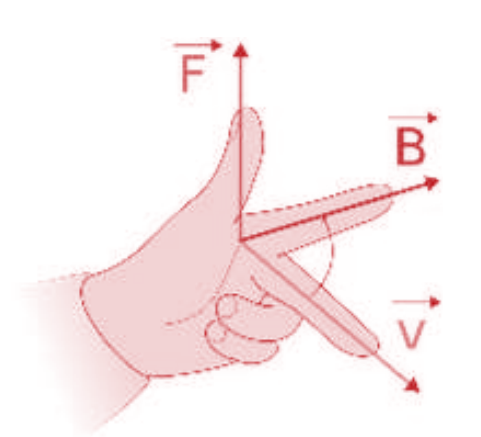
\includegraphics[width=0.6\linewidth]{mano_izquierda.png}
    \end{center}
    \begin{itemize}
      \item Pulgar: $\vec{F}$
      \item Índice: $\vec{B}$
      \item Medio: $\vec{v}$
    \end{itemize}
    \footnotesize\textit{Válido para $q > 0$; invertir para $q < 0$ (Usa la mano derecha en ese caso.)}
  \end{notabox}

\end{multicols}

\end{document}